\documentclass{article}
\usepackage[a4paper,top=3cm,bottom=2.5cm,left=2.5cm,
            right=2cm,marginparwidth=1.75cm,
            headheight=5pt]{geometry}
\usepackage[T5]{fontenc}
\usepackage[utf8]{inputenc}
\usepackage[document]{ragged2e}
\usepackage[vietnamese]{babel}
\usepackage[unicode]{hyperref}
\usepackage{amsmath}
\usepackage{setspace}
\usepackage{graphicx}
\usepackage{caption}
\usepackage{subcaption}
\usepackage{tcolorbox}
\usepackage{listings}
\usepackage{hyperref}
\usepackage{xcolor}
\usepackage{longtable}
\usepackage{titlesec}
\usepackage{floatrow}
\usepackage[nottoc]{tocbibind}
\usepackage{mdframed}
\usepackage{amsmath}
\usepackage{amssymb}
\usepackage{tgbonum}
\usepackage{type1cm}
\usepackage{indentfirst}
\usepackage{lettrine}
\usepackage{colortbl}
\usepackage{fancyhdr}
\usepackage{wrapfig}
\usepackage{lastpage}
\usepackage{url}
\addto\captionsenglish{
  \renewcommand{\contentsname}{MỤC LỤC}%
  \renewcommand{\listfigurename}{Danh sách ảnh}%
  \renewcommand{\listtablename}{Danh sách bảng}%
  \renewcommand{\figurename}{Hình}
  \renewcommand{\tablename}{Bảng}
}
\pagestyle{fancy}
\fancyhf{}
\rhead{Toán ứng dụng và thống kê}
\lhead{\color{cyan}Đồ án 2: Image Processing}
\lfoot{Trang \thepage /\pageref{LastPage}}
\renewcommand{\footrulewidth}{0.4pt}
\setlength{\parindent}{5pt}
\setlength{\parskip}{1cm}
\renewcommand{\baselinestretch}{1.5}
\newmdenv[linecolor=black,skipabove=\topsep,skipbelow=\topsep,
leftmargin=2.5cm,rightmargin=2.5cm,
innerleftmargin=5cm,innerrightmargin=5cm]{mybox}
\usepackage{multicol}
\usepackage{indentfirst}
\usepackage{color}
\usepackage{apacite}
\usepackage{tikz}
\graphicspath{{Figures/}} 
\usepackage[square, numbers, comma, sort&compress]{natbib}  
\usepackage{lipsum}
\usetikzlibrary{calc}
\setlength{\columnseprule}{2pt}
\def\columnseprulecolor{\color{black}}
\def\maru#1{\textcircled{\scriptsize#1}}

\begin{document}
% Bìa trang
\begin{titlepage}
\begin{tikzpicture}[remember picture,overlay,inner sep=0,outer sep=0]
     \draw[blue!70!black,line width=4pt] ([xshift=-1.5cm,yshift=-2cm]current page.north east) coordinate (A)--([xshift=2cm,yshift=-2cm]current page.north west) coordinate(B)--([xshift=2cm,yshift=2cm]current page.south west) coordinate (C)--([xshift=-1.5cm,yshift=2cm]current page.south east) coordinate(D)--cycle;

     \draw ([yshift=0.5cm,xshift=-0.5cm]A)-- ([yshift=0.5cm,xshift=0.5cm]B)--
     ([yshift=-0.5cm,xshift=0.5cm]B) --([yshift=-0.5cm,xshift=-0.5cm]B)--([yshift=0.5cm,xshift=-0.5cm]C)--([yshift=0.5cm,xshift=0.5cm]C)--([yshift=-0.5cm,xshift=0.5cm]C)-- ([yshift=-0.5cm,xshift=-0.5cm]D)--([yshift=0.5cm,xshift=-0.5cm]D)--([yshift=0.5cm,xshift=0.5cm]D)--([yshift=-0.5cm,xshift=0.5cm]A)--([yshift=-0.5cm,xshift=-0.5cm]A)--([yshift=0.5cm,xshift=-0.5cm]A);


     \draw ([yshift=-0.3cm,xshift=0.3cm]A)-- ([yshift=-0.3cm,xshift=-0.3cm]B)--
     ([yshift=0.3cm,xshift=-0.3cm]B) --([yshift=0.3cm,xshift=0.3cm]B)--([yshift=-0.3cm,xshift=0.3cm]C)--([yshift=-0.3cm,xshift=-0.3cm]C)--([yshift=0.3cm,xshift=-0.3cm]C)-- ([yshift=0.3cm,xshift=0.3cm]D)--([yshift=-0.3cm,xshift=0.3cm]D)--([yshift=-0.3cm,xshift=-0.3cm]D)--([yshift=0.3cm,xshift=-0.3cm]A)--([yshift=0.3cm,xshift=0.3cm]A)--([yshift=-0.3cm,xshift=0.3cm]A);

   \end{tikzpicture}
\newcommand{\HRule}{\rule{\linewidth}{0.5mm}}
\center

\textsc{\Large TRƯỜNG ĐẠI HỌC KHOA HỌC TỰ NHIÊN}\\[0.5cm]
\textsc{\Large KHOA CÔNG NGHỆ THÔNG TIN}\\[1cm]

\includegraphics[width=0.3\textwidth]{logo/KHTN.jpg}\\[1cm]

\HRule \\[0.4cm]
{\huge \bfseries ĐỒ ÁN 2: IMAGE PROCESSING} \\[0.4cm]
{\large TOÁN ỨNG DỤNG VÀ THỐNG KÊ}\\[0.1cm]
\HRule \\[1.5cm]

\centerline{\Large{\textbf{Triệu Nhật Minh — 21127112 — 21CLC02}}}
\vspace{2.5cm}
\centerline{\large{\textit{Giảng viên hướng dẫn}}}
\vspace{0.25cm}
\centerline{\large{Vũ Quốc Hoàng}}
\centerline{\large{Lê Thanh Tùng}}
\centerline{\large{Nguyễn Văn Quang Huy}}
\centerline{\large{Phan Thị Phương Uyên}}

\vspace{2.5cm}
\centerline{\today}


\vfill % Wipe blank space of the page.
\end{titlepage}

% Mục lục tự động
\setlength{\parskip}{.7em}
\tableofcontents
\newpage

% Table of Figures & Tables
\setlength{\parskip}{.5em}
%\listoffigures
%\listoftables
\newpage

% Bắt đầu nội dung
\section{Hướng dẫn sử dụng}
\begin{description}
  \item[Bước 1:] Run all các cell trong notebook \textbf{21127112.ipynb} (hoặc chỉ run cell cuối cùng để chạy hàm main nếu đã khởi chạy các hàm bổ trợ từ trước).
  \item[Bước 2: ] Nhập đường dẫn tới ảnh cần xử lý (chỉ cần tên ảnh nếu ảnh đã nằm cùng thư mục với notebook).
  \item[Bước 3: ] Chọn chức năng cần thực hiện (từ 0-8 tương ứng với các chức năng và 9 để thoát chương trình).
  \item[Bước 4: ] 
\end{description}

\section{Đánh giá kết quả}
\begin{longtable}[c]{|r|l|c|l|}
  \hline
  \rowcolor[HTML]{00D2CB} 
  \multicolumn{1}{|c|}{\cellcolor[HTML]{00D2CB}{\color[HTML]{FFFFFF} \textbf{STT}}} & \multicolumn{1}{c|}{\cellcolor[HTML]{00D2CB}{\color[HTML]{FFFFFF} \textbf{Chức năng}}} & {\color[HTML]{FFFFFF} \textbf{Mức độ hoàn thành}} & \multicolumn{1}{c|}{\cellcolor[HTML]{00D2CB}{\color[HTML]{FFFFFF} \textbf{Kết quả}}} \\ \hline
  \endfirsthead
  %
  \endhead
  1 & Thay đổi độ sáng cho ảnh & 100\% & \parbox[c]{8em}{\includegraphics[width=8em]{image/lena_brightness_128.png}} \\ \hline
  2 & Thay đổi độ tương phản & 100\% & \parbox[c]{8em}{\includegraphics[width=8em]{image/lena_contrast_128.png}} \\ \hline
  3 & Lật ảnh ngang & 100\% & \parbox[c]{8em}{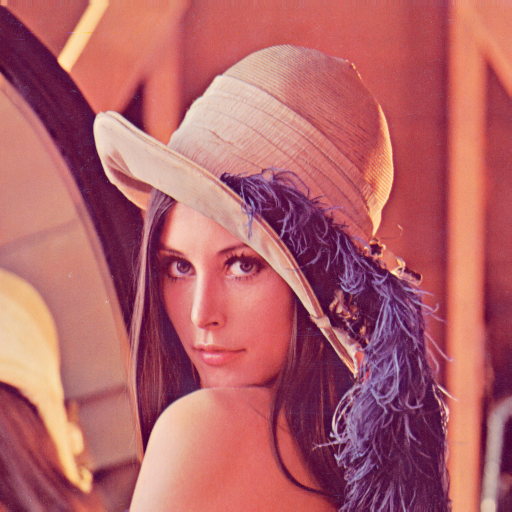
\includegraphics[width=8em]{image/lena_flip_horizontal.png}} \\ \hline
  4 & Lật ảnh dọc & 100\% & \parbox[c]{8em}{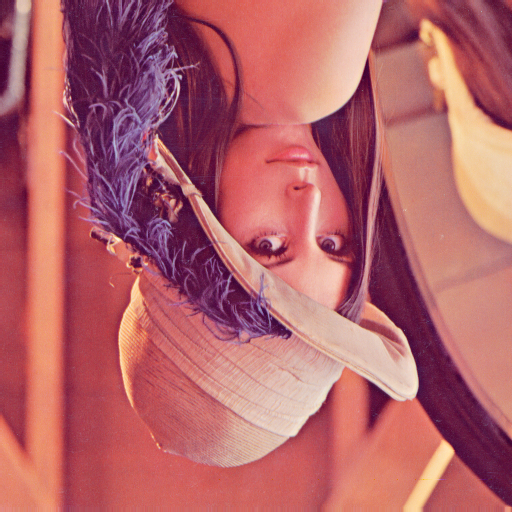
\includegraphics[width=8em]{image/lena_flip_vertical.png}} \\ \hline 
  5 & Chuyển đổi thành ảnh xám & 100\% & \parbox[c]{8em}{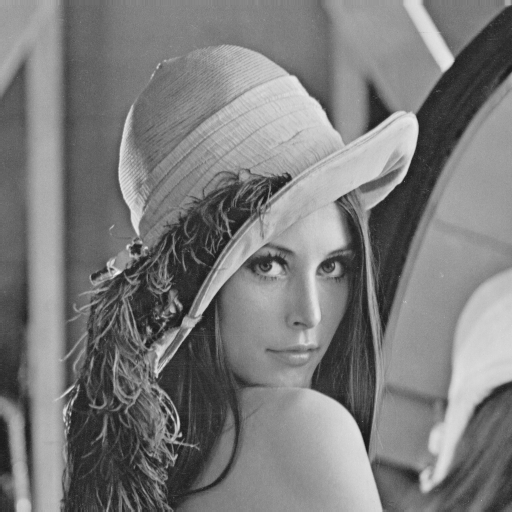
\includegraphics[width=8em]{image/lena_grayscale.png}} \\ \hline
  6 & Chuyển đổi thành ảnh sepia & 100\% & \parbox[c]{8em}{\includegraphics[width=8em]{image/lena_sepia.png}} \\ \hline
  7 & Làm mờ & 100\% & \parbox[c]{8em}{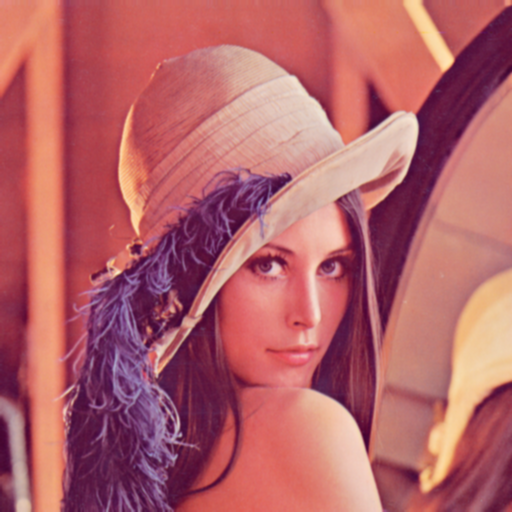
\includegraphics[width=8em]{image/lena_blur.png}} \\ \hline
  8 & Làm sắc nét ảnh & 100\% & \parbox[c]{8em}{\includegraphics[width=8em]{image/lena_sharpen.png}} \\ \hline
  9 & Cắt ảnh theo kích thước (cắt ở trung tâm) & 100\% & \parbox[c]{8em}{\includegraphics[width=8em]{image/lena_center_crop.png}} \\ \hline
  10 & Cắt ảnh theo khung hình tròn & 100\% & \parbox[c]{8em}{\includegraphics[width=8em]{image/lena_circular_crop.png}} \\ \hline
  11 & Cắt ảnh theo khung elip & 100\% & \parbox[c]{8em}{\includegraphics[width=8em]{image/lena_elliptical_crop.png}} \\ \hline
\end{longtable}

% \begin{table}[ht] 
%   \centering
%   \begin{tabular}{|l|l|l|l|l|} \hline 
%       Stimuli Category & Familiar Organism & Growth Model & Metamorphosis & Figure \\ \hline
%       \textbf{FDM} & Yes & Dramatic & Yes & \parbox[c]{7em}{\includegraphics[width=0.15\textwidth]{image/lena_brightness_128.png}} \\ \hline
%   \end{tabular}
% \end{table}

\section{Mô tả}
\textcolor{red}{Để thuận tiện cho phần trình bày bên dưới, từ bây giờ, mỗi điểm ảnh gồm 3 giá trị của kênh màu RGB sẽ được xem như một phần tử màu. Do đó, ma trận các điểm ảnh được xem như mảng 2 chiều các điểm ảnh, kí hiệu: \textit{img\_2d}. }
% Template mô tả hàm
% \textbf{Input:} \\
% \textbf{Output:}

% \paragraph{Mô tả:}
\subsection{Nhóm hàm chính}
\subsubsection{Hàm change\_brightness}
\textbf{Input:} Mảng NumPy 2 chiều các điểm ảnh \textit{img\_2d}, giá trị độ sáng \textit{brightness} (mặc định là 128 nếu không truyền tham số vào hàm). \\
\textbf{Output:} Mảng NumPy 2 chiều các điểm ảnh, chuỗi kí tự chứa hậu tố của tên file ảnh sau xử lý.

\paragraph{Ý tưởng thực hiện:} Thay đổi độ sáng bức ảnh là cùng lúc thay đổi giá trị trong phần tử màu của từng pixel ảnh cho một hằng số. Bức ảnh sau khi thay đổi độ sáng sẽ có màu sáng hơn hoặc tối hơn tùy thuộc vào giá trị của hằng số này, càng tối nghĩa là càng nhiều pixel có giá trị màu gần 0 và ngược lại.

\paragraph{Mô tả:} Để thay đổi độ sáng của ảnh, ta chỉ cần cộng thêm giá trị \textit{brightness} vào mỗi giá trị trong phần tử màu của mảng \textit{img\_2d}. Tuy nhiên, giá trị này có thể vượt quá khoảng giá trị cho phép của một giá trị của phần tử màu (từ 0 đến 255). Do đó, trước khi thực hiện phép cộng, ta cần đổi kiểu dữ liệu của mảng \textit{img\_2d} thành int64 để có thể lưu được các giá trị nguyên âm và giá trị nguyên dương lớn hơn 255. Sau khi thực hiện xong, kết hợp việc giới hạn giá trị sử dụng hàm \textit{limit\_value} và ép kiểu dữ liệu về uint8, ta được mảng 2 chiều các điểm ảnh sau khi thay đổi độ sáng.

\subsubsection{Hàm change\_contrast}


\subsubsection{Hàm flip\_image}
\subsubsection{Hàm convert\_grayscale}
\subsubsection{Hàm convert\_sepia}
\subsubsection{Hàm convolute\_2D}
\subsubsection{Hàm blur\_image / sharpen\_image}
\subsubsection{Hàm center\_crop}
\subsubsection{Hàm circular\_crop}
\subsubsection{Hàm elliptical\_crop}

\subsection{Nhóm hàm bổ trợ}
\subsubsection{Hàm limit\_value}
\subsubsection{Hàm show\_image}
\subsubsection{Hàm write\_image}
\subsubsection{Hàm read\_image}
\subsubsection{Hàm main}

\newpage
\subsection{Nhận xét}
\subsubsection{Về ảnh đầu ra}

\subsubsection{Về tài nguyên sử dụng}

\centerline{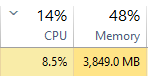
\includegraphics[width=0.2\textwidth]{image/performance.png}}
\newpage
\section{Tài liệu tham khảo}
\begin{itemize}
    \item \href{https://matplotlib.org/stable/api/_as_gen/matplotlib.pyplot.figure.html}{matplotlib.pyplot.figure}
    \item \href{https://numpy.org/doc/stable/user/basics.broadcasting.html}{Broadcasting explained}
\end{itemize}

\end{document}